\chapter{Results and Discussion}
\begin{refsection}

This chapter discusses the results and evaluation of the Retrieval-Augmented Generation (RAG) chatbot developed for efficient literature search and thesis retrieval at the Camarines Sur Polytechnic Colleges (CSPC) Library.

\subsection{Dataset and Preparation}
The study corpus comprised all available undergraduate thesis PDFs from multiple CSPC departments (290+ documents). Coordination with the CSPC Library established data handling practices and local/on-premise deployment. The dataset was prepared via structured text extraction and token-based chunking aligned with thesis sections (Abstract; Chapters 1--5), enabling section-aware retrieval.


\begin{figure}[h]
    \centering
    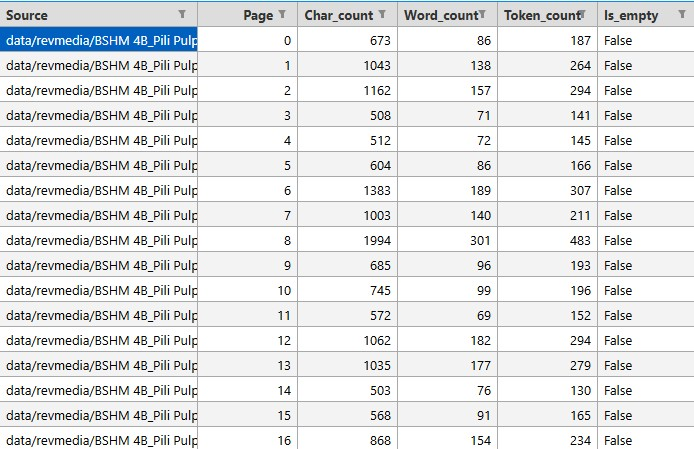
\includegraphics[width=0.7\textwidth]{figures/doc_analysis.jpg}
    \caption{CSPC Thesis PDF Analysis}
\end{figure}

Upon agreement on project scope, data handling practices, and local/on-premise deployment, library personnel granted the researchers to gain access to the digital copies of undergraduate thesis papers. The dataset was acknowledged and queued for the development phase following the proposed model pipelines’ process.

\subsection{Data Preprocessing}
Texts were extracted page-by-page and enriched with metadata (source, page) to preserve academic provenance. Token-based chunking produced coherent segments sized to the LLM context window and guided by thesis structure, improving retrieval fidelity and citation transparency.

\begin{figure}[h]
    \centering
    \begin{minipage}{0.48\textwidth}
        \centering
        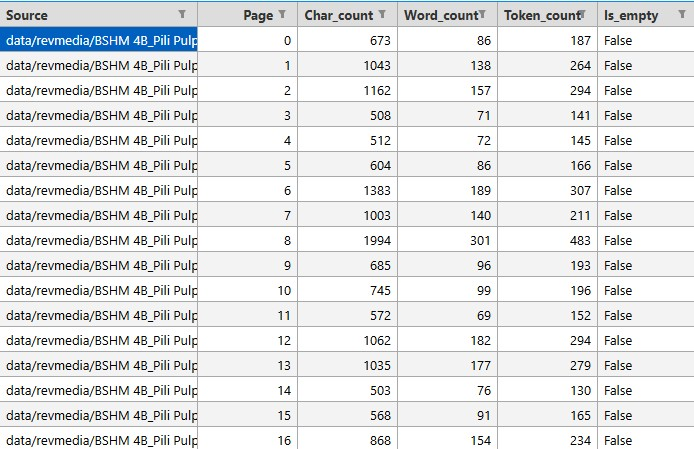
\includegraphics[width=0.95\textwidth]{figures/chunk_analysis.jpg}
        \caption{Chunk Analysis}
    \end{minipage}\hfill
    \begin{minipage}{0.48\textwidth}
        \centering
        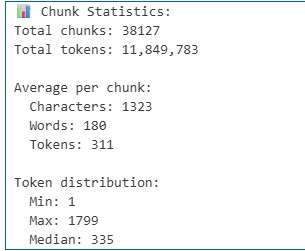
\includegraphics[width=0.75\textwidth]{figures/chunk_stat.jpg}
        \caption{Chunk Statistics}
    \end{minipage}
\end{figure}

This preprocessing yielded clean, contextually rich segments suitable for vectorization and indexing.    

\subsection{Indexing and Vector Database Construction}
The indexing phase transformed the preprocessed text chunks into a searchable knowledge base optimized for semantic retrieval within the RAG pipeline. This critical stage bridged the gap between raw textual content and the intelligent query-response capabilities that would define the chatbot's effectiveness in academic literature discovery.

\begin{figure}[h]
    \centering
    
\includegraphics[width=0.7\textwidth]{figures/index.jpg}
    \caption{Created index in FAISS}
\end{figure}

Embeddings were generated primarily with sentence-transformers/all-MiniLM-L6-v2 (HuggingFace), chosen for its efficiency and strong semantic performance; when cloud embeddings were available, Gemini could be used as an alternative for multilingual scenarios. FAISS stored vectors alongside source/page metadata to preserve traceability. This enabled natural language queries to retrieve semantically relevant thesis segments beyond exact keyword matching.

\subsection{Query Encoding and Retrieval}
Queries were embedded using the same model as indexing to ensure consistency. The FAISS-backed retriever returned the top-$K$ relevant chunks (default $K=6$), balancing precision and recall. Diversity-enhancing strategies (e.g., MMR) were used for broader queries to avoid redundant chunks.

For example, when users asked, “What research has been done on machine learning applications in healthcare?” or “Show me theses about sustainable energy solutions,” the system retrieved abstracts and key sections.  Notably, setting $K=6$ produced a good balance of focused context and cross-thesis coverage.

\subsection{Augmented Input and Generation}
Retrieved chunks were concatenated with the user query into a structured context with lightweight citation markers (e.g., source filename, page). This supported grounded, traceable answers and reduced hallucination risk.

Prompt templates guided the model to answer strictly from provided context, with safeguards (token monitoring, truncation) to maintain input quality.

\subsection{Response Generation}

The Gemini 2.5-flash model generated answers grounded in retrieved context. The system was configured with temperature=0 to ensure deterministic outputs suitable for academic use.
 
Generated content was parsed into clean text for display. While RAG significantly reduced hallucinations, occasional inaccuracies were observed when context was insufficient; users were advised to validate critical findings.

\section{Interface and Usage Observations}

The Streamlit interface supported conversational exploration with session-based history and safety filters for disallowed queries. Cached chains ensured responsive interactions.

\begin{figure}[h]
    \centering
    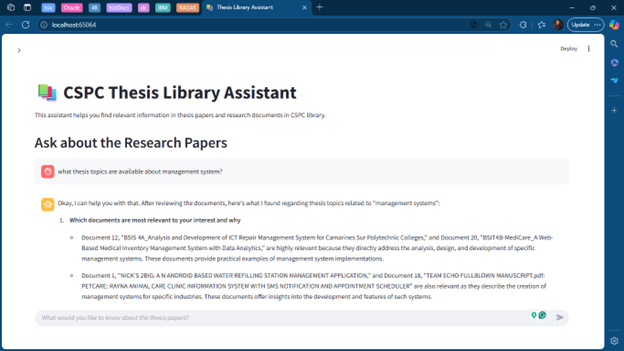
\includegraphics[width=0.7\textwidth]{figures/streamlit.png}
    \caption{Streamlit Interface Display}
\end{figure}

Generated responses appeared as Markdown with citations and structured text. When queries violated safety parameters, clear warnings were shown. Deterministic settings improved consistency and user trust.

\section{Model Evaluation}
In this section, the RAG-based chatbot system for the CSPC Library was evaluated utilizing four critical metrics: Answer Relevancy, Context Precision, Context Recall, and Faithfulness. These metrics provide a multidimensional perspective on the performance of the literature retrieval system, ensuring robust analysis in both information quality and reliability. The evaluation framework and explanations are patterned after established academic standards as demonstrated in the reference thesis.

\section{Result}
This section presents the findings through tables, figures, and subsequent discussion. Prior to evaluation, a systematic data processing pipeline was applied: 290+ undergraduate thesis PDFs from the CSPC Library were processed into segmented meaningful text chunks, and embedded using Hugging Face's Embeddings. These chunks were indexed in FAISS for efficient semantic retrieval, enabling the RAG chatbot to generate contextually relevant and factually grounded responses for user queries. This process ensured that the evaluation was conducted on high-quality, well-structured academic data. In addition to the system-level RAGAS metrics, a complementary user-centered evaluation was performed using a 5-point Likert scale questionnaire, responses were summarized via weighted mean and interpreted using predefined agreement ranges (see \ref{tab:likert_scale}) to align technical performance with perceived usability and satisfaction.

\begin{table}[H]
    \centering
    \caption{RAG System Evaluation Metrics using RAGAS Framework}
    \label{tab:rag_metrics}
    \begin{tabular}{ll} 
        \hline
        \textbf{Metric}     & \textbf{Average Score} \\
        \hline
        Answer Relevancy    & 0.737 \\
        Context Precision   & 0.818 \\
        Context Recall      & 0.721 \\
        Faithfulness        & 0.585 \\
        \hline
    \end{tabular}
\end{table}

The table presented above provides a concise summary of the RAG system’s evaluation metrics, offering a clear view of its performance in literature search and thesis retrieval tasks. Each metric captures a distinct aspect of the system’s effectiveness:

\begin{enumerate}
\item \textbf{Answer Relevancy (0.737):} This metric reflects how well the system’s responses address user queries. A score of 0.737 indicates that the chatbot generally provides answers that are relevant and useful, supporting users in finding the information they seek.
\item \textbf{Context Precision (0.818):} Context precision measures the proportion of retrieved text chunks that are actually relevant to the query. With a high score of 0.818, the system demonstrates strong ability to filter out irrelevant information, ensuring that users receive focused and meaningful content.
\item \textbf{Context Recall (0.721):} This metric assesses the system’s ability to retrieve all relevant information needed to answer a query. A score of 0.721 suggests that the chatbot successfully gathers most of the necessary supporting content, though there is still room for improvement in capturing every relevant detail.
\item \textbf{Faithfulness (0.585):} Reflects how accurately the chatbot's generated responses were supported by the source documents. While lower than other metrics, this value highlights a key area for improvement, emphasizing the challenge of maintaining strict factual consistency in generative retrieval systems.
\end{enumerate}

\noindent These metrics offer a comprehensive view of the system’s effectiveness. High answer relevancy and context precision demonstrate the chatbot’s practicality and efficiency in delivering relevant results, while context recall and faithfulness underscore the system’s coverage and reliability. Faithfulness, in particular, remains an ongoing focus for enhancement, aligning with current research advances in AI literature retrieval. These metrics collectively form the foundation for interpreting, tuning, and extending the RAG chatbot’s capabilities within the CSPC Library environment.

\begin{figure}[h]
    \centering
    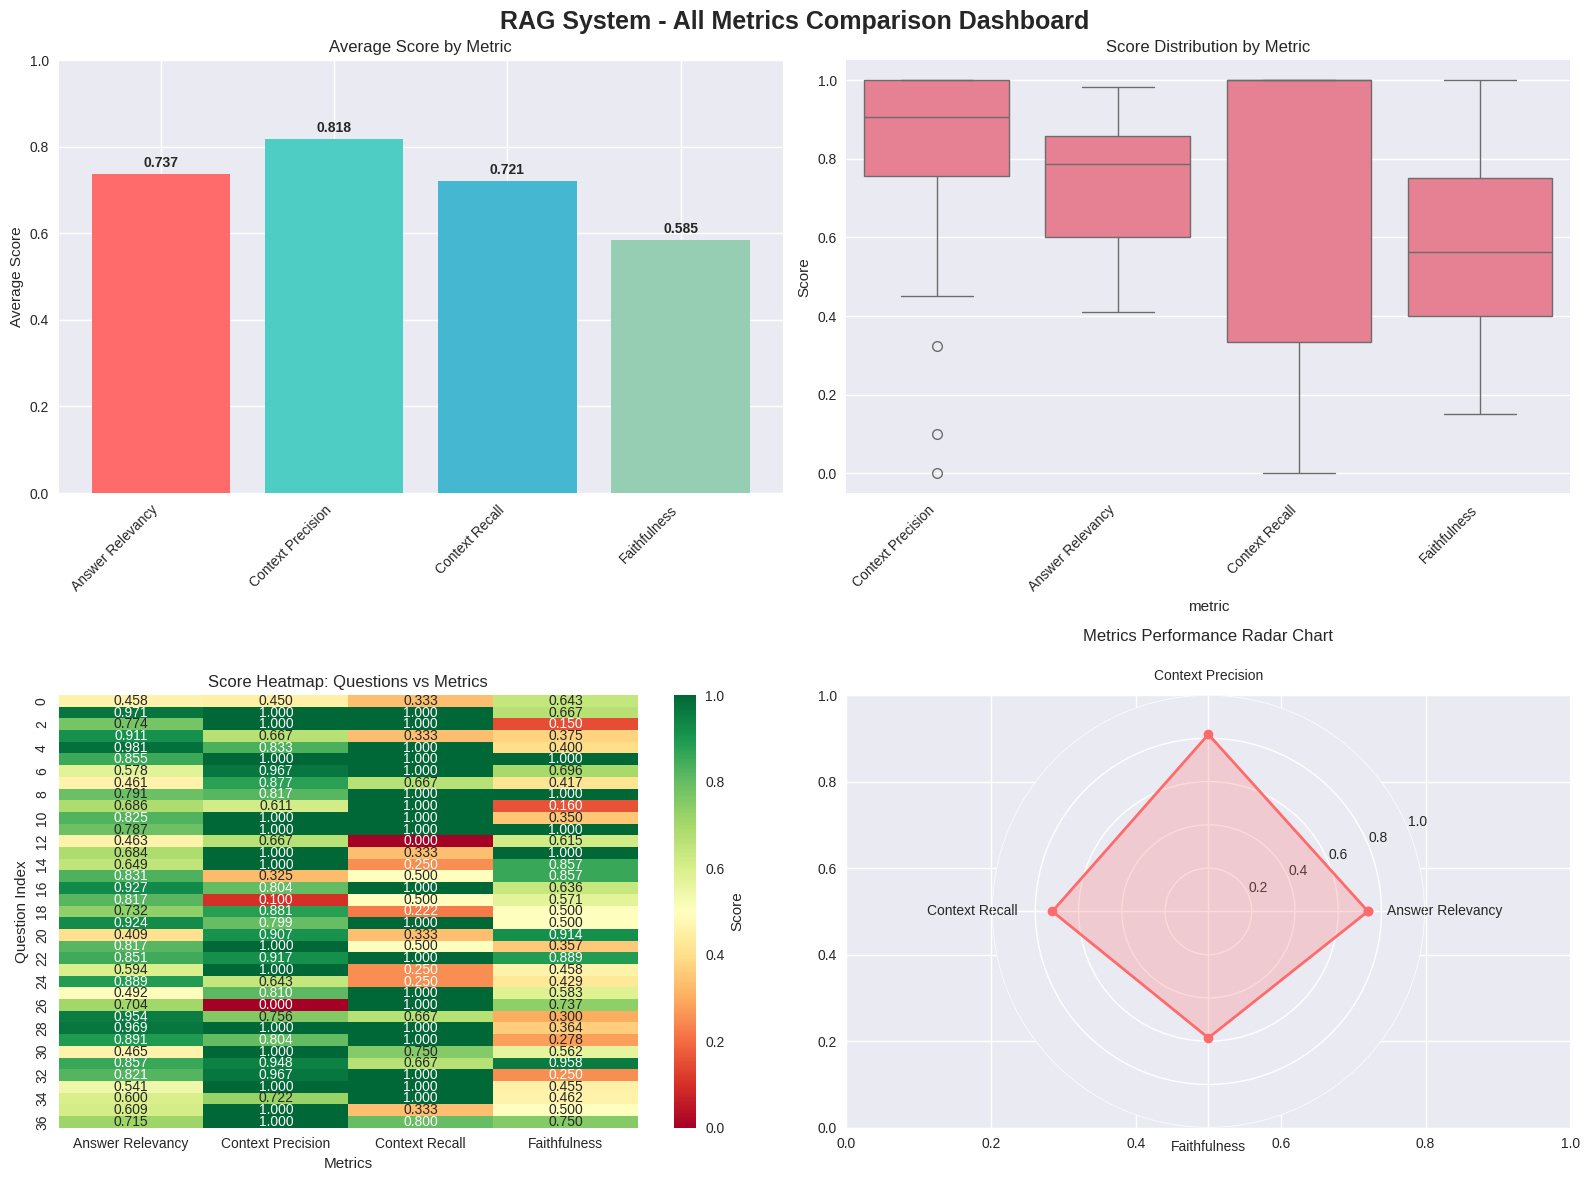
\includegraphics[width=0.7\textwidth]{figures/overall_out.png}
    \caption{RAG System - Metrics Dashboard}
\end{figure}

\section*{RAG System - Metrics Dashboard}
The dashboard presented herein serves as an integrated visualization tool for evaluating the RAG system’s performance across four core metrics: Answer Relevancy, Context Precision, Context Recall, and Faithfulness. Each chart within the dashboard offers unique insights into different aspects of system behavior in the context of literature search and thesis retrieval.
The bar chart illustrates the average score attained for each metric. Notably, Context Precision achieves the highest average (0.818), followed by Answer Relevancy (0.737), Context Recall (0.721), and Faithfulness (0.585). This ordering highlights the system’s exceptional ability to retrieve relevant information, moderate competence in delivering complete and relevant answers, and a comparative need for improvement in grounding generated responses strictly within the source material.
The box plot details the score distribution across metrics, emphasizing both consistency and spread. Metrics such as Context Precision and Answer Relevancy display less variance and higher minimum scores, indicating stable system performance. In contrast, Context Recall and Faithfulness exhibit a broader range, evidencing occasional lapses in comprehensive retrieval and accurate grounding.
The heatmap provides a granular view by displaying metric scores for individual questions. Darker shades correspond to higher scores, meaning better performance for both retrieval and generation on those specific queries. The heatmap reveals that while the chatbot excels on many questions, there is still inconsistency—some queries show lower faithfulness or recall, suggesting targets for further system refinement.
The radar chart synthesizes the metric scores into a single shape, depicting the RAG system’s overall performance profile at a glance. The profile is robust in Context Precision and Answer Relevancy, slightly reduced in Context Recall, and tapers at Faithfulness. This visualization makes clear where the system currently excels and where enhancements should be prioritized.

These visualizations collectively deliver a comprehensive, multi-faceted overview of the RAG chatbot’s strengths and areas for further enhancement. The visualizations reveal the system’s strong retrieval precision and relevancy, adequate recall, and opportunities for improvement regarding faithfulness to source documents. These insights guide ongoing refinements to optimize the chatbot for reliable, accurate, and comprehensive academic information retrieval.

\section*{User Agreement on Chatbot Response Quality and Performance}
\ref{tab:user_agreement_quality} shows the results of the user-centered evaluation of the CSPC Library RAG chatbot using 5-point likert scale survey questions that allows the respondents to evaluate and choose the level of agreement with the chatbot’s response quality and performance.

\begin{table}[H]
    \centering
    \caption{User Agreement: Chatbot Response Quality and Performance}
    \label{tab:user_agreement_quality}
    \begin{tabular}{p{7cm} c c}
        \hline
        \multicolumn{1}{c}{\textbf{Criteria}} & \textbf{Weighted Mean} & \textbf{Verbal Interpretation} \\
        \hline
        The questions are answered well by the chatbot. & 4.3 & Strongly Agree \\
        \hline
        The answers are relevant to the question. & 4.5 & Strongly Agree \\
        \hline
        Chatbot’s responses are clear and understandable. & 4.5 & Strongly Agree \\
        \hline
        The chatbot’s responses help answer your questions. & 4.3 & Strongly Agree \\
        \hline
        The chatbot provided enough information. & 4.2 & Strongly Agree \\
        \hline
        The chatbot has a quick response time. & 4.1 & Agree \\
        \hline
        \textbf{Overall Weighted Mean} & \textbf{4.3} & \textbf{Strongly Agree} \\
        \hline
    \end{tabular}
\end{table}

The result of the evaluation of the RAG chatbot using user-centered evaluation method indicate a generally positive reception from users across various criteria. Here’s the breakdown of the findings. In terms of the chatbot’s question and answering performance, users strongly agreed (weighted mean: 4.3) that the system performed well in answering user questions, indicating that the chatbot meets user expectation in getting right answers. Users also strongly agreed (weighted mean: 4.5) that the chatbot provide answers relevant to the questions provided by the users, indicating that the system effectively interprets user intent and provide relevant answers based on the questions. Furthermore, users strongly agreed (weighted mean: 4.5) that the chatbot gives clear and easy-to-understand answers. This means the chatbot not only gives correct responses but also explains them in a way that users can easily follow. Moreover, the chatbot helped users find the answers they were looking for. With a (weighted mean of 4.3), users strongly agreed that the chatbot’s replies were useful and matched their questions well. This shows that the system supports users in getting the help they need. In the same way, the chatbot provided enough information to help users, with a weighted mean of 4.2. This shows that users  strongly agreed and felt the chatbot gave complete and useful answers during their interaction. Lastly, the chatbot was quick to reply, with users agreeing (weighted mean: 4.1) that it responded without delay. This means the system was able to give answers fast, helping users get the information they needed right away. Overall, the respondents showed agreement across the measured areas, with an average weighted mean of 4.3 (Strongly Agree). This indicates that users found the chatbot’s answers to be correct, relevant, clear, and mostly complete, and that the chatbot responded quickly enough to be useful These findings suggest the chatbot works well for its main task of helping users find information and understand answers. Minor improvements could focus on making responses more complete and slightly faster to raise overall satisfaction even more. Furthermore, according to \citeauthor{folstad2021future} \citeyear{folstad2021future}, user-centered evaluation has been key within several disciplines at the roots of current chatbot research, particularly in understanding users' needs, motivations, and experiences with chatbot interactions. Thus, it is advisable to utilize this method to assess system effectiveness and user satisfaction before deployment to ensure the RAG chatbot meets actual user expectations and provides satisfactory support for thesis retrieval tasks in the CSPC Library context.

\section*{User Feedback on RAG chatbot’s Effectiveness and Usability}
\ref{tab:user_feedback_table} presents the user-centered evaluation results of the RAG chatbot using a 5-point Likert scale. The table shows weighted means for user satisfaction, likelihood of using the chatbot again, ease of reading and understanding the chatbot’s output, and confidence in the chatbot’s information, allowing readers to gauge overall user perception and intent to use the system in the future.

\begin{table}[H]
    \centering
    \caption{User Feedback on RAG chatbot’s Effectiveness and Usability}
    \label{tab:user_feedback_table}
    \begin{tabular}{m{5cm} c c}
        \hline
        \multicolumn{1}{c}{\textbf{Criteria}} & \textbf{Weighted Mean} & \textbf{Verbal Interpretation} \\
        \hline
        Satisfaction with answers & 4.1 & Satisfied \\
        \hline
        Likelihood of using the chatbot again & 4.3 & Very Likely \\
        \hline
        Ease of understanding the chatbot’s output & 4.5 & Very Easy \\
        \hline
        Confidence in the chatbot’s information & 3.8 & Confident \\
        \hline
    \end{tabular}
\end{table}

The results for satisfaction with answers, likelihood to use again, ease of reading and understanding, and confidence in information accuracy show generally positive user feedback. And, according to \citeauthor{kaushal2022role} \citeyear{kaushal2022role} and \citeauthor{okonkwo2021chatbots} \citeyear{okonkwo2021chatbots}, these aspects of chatbots that deliver clear, useful, and readable responses greatly improve user satisfaction. In addition, \citeauthor{choudhury2023investigating} \citeyear{choudhury2023investigating} and \citeauthor{zhang2024ai} \citeyear{zhang2024ai} found that trust and factual accuracy are essential for encouraging continued use and building user confidence in AI chatbots. After considering these established determinants, the detailed breakdown is as follows. In terms of user satisfaction with answers, users were satisfied (weighted mean: 4.1), indicating that the chatbot’s replies met users’ needs and were generally acceptable. Regarding likelihood of reuse, users were very likely to use the chatbot again (4.3), suggesting strong perceived utility. Users also found the responses very easy to read and understand (4.5), demonstrating clear and user-friendly output. Confidence in the chatbot’s information was moderately strong (3.8), implying general trust with some expectation for accuracy improvements. Overall, the respondents provided positive feedback across all measures, showing that the chatbot delivers useful, relevant, clear, and mostly complete answers, supports continued usage intention, and yields satisfactory user experience, with factual confidence identified as a targeted area for further enhancement.

%=======================================================%
%%%%% Do not delete this part %%%%%%
\clearpage

\printbibliography[heading=subbibintoc, title={\centering Notes}]
\end{refsection}